\documentclass[letterpaper,10pt]{article}

\usepackage{titling}
\usepackage{listings}
\usepackage{url}
\usepackage{setspace}
\usepackage{subfig}
\usepackage{sectsty}
\usepackage{pdfpages}
\usepackage{colortbl}
\usepackage{multirow}
\usepackage{multicol}
\usepackage{relsize}
\usepackage{amsmath}
\usepackage{wasysym}
\usepackage{fancyvrb}
\usepackage{amssymb}
\usepackage{ifsym}
\usepackage{amsmath,amssymb,amsthm,graphicx,xspace}
\usepackage[titlenotnumbered,noend,noline]{algorithm2e}
\usepackage[compact]{titlesec}
\usepackage{XCharter}
\usepackage[T1]{fontenc}
\usepackage{tikz}
\usetikzlibrary{arrows,automata,shapes,trees,matrix,chains,scopes,positioning,calc}
\tikzstyle{block} = [rectangle, draw, fill=blue!20, 
    text width=2.5em, text centered, rounded corners, minimum height=2em]
\tikzstyle{bw} = [rectangle, draw, fill=blue!20, 
    text width=4em, text centered, rounded corners, minimum height=2em]

\definecolor{namerow}{cmyk}{.40,.40,.40,.40}
\definecolor{namecol}{cmyk}{.40,.40,.40,.40}

\let\LaTeXtitle\title
\renewcommand{\title}[1]{\LaTeXtitle{\textsf{#1}}}


\newcommand{\handout}[5]{
  \noindent
  \begin{center}
  \framebox{
    \vbox{
      \hbox to 5.78in { {\bf ECE356: Database Systems } \hfill #2 }
      \vspace{4mm}
      \hbox to 5.78in { {\Large \hfill #4  \hfill} }
      \vspace{2mm}
      \hbox to 5.78in { {\em #3 \hfill} }
    }
  }
  \end{center}
  \vspace*{4mm}
}

\newcommand{\lecture}[3]{\handout{#1}{#2}{#3}{Lecture #1}}
\newcommand{\tuple}[1]{\ensuremath{\left\langle #1 \right\rangle}\xspace}

\addtolength{\oddsidemargin}{-1.000in}
\addtolength{\evensidemargin}{-0.500in}
\addtolength{\textwidth}{2.0in}
\addtolength{\topmargin}{-1.000in}
\addtolength{\textheight}{1.75in}
\addtolength{\parskip}{\baselineskip}
\setlength{\parindent}{0in}
\renewcommand{\baselinestretch}{1.5}
\newcommand{\term}{Winter 2018}

\singlespace


\begin{document}

\lecture{ 7 --- Security }{\term}{Jeff Zarnett}

\section*{Security, Report to the Bridge}

In a lot of books, and even in my original plan for how the lectures would be carried out, security was left to the end. This strikes me as being a disservice: security is something you want to bake into your product and something you want to have in your mind when you are designing it. It doesn't work to try to bolt it on afterwards. 

Just as a matter of terminology: an \textit{attacker} is a malicious user who is trying to damage or exploit the system. A \textit{countermeasure} is some action or process we can take or implement to defend against attacks. An attacker is successful if he or she gains access to information he/she shouldn't have, damages the system in some way, or interferes with its legitimate operations.

In this lecture we will not go into the legal or ethical issues related to security, or security policies that are designed by organizations to tell you what keeps the system secure. We will focus on how access is controlled in the database, and specifically about the SQL Injection attack. 

The truth is that databases contain a lot of data and some of it might be sensitive. In fact, there are several ways a piece of data could be declared sensitive. It might be that it is personal information, such as medical history of a patient or an employee's home address. It could also be that it comes from a sensitive source. The sensitive data might not be the entire tuple; it might just be a particular attribute  such as Social Security Number or salary~\cite{fds}. 

Regardless of why some data is sensitive, database administrators must see to it that the security policies are enforced. This means specifically that sensitive data is protected, but also that data is not corrupted and that access to any data is limited to those who should have access. Security policies do have some tradeoff with usability in that it can be frustrating for users who are denied some operation and must instead ask administrators to do it for them. But you also can't be too lax about this, because you most certainly do NOT want to find your company's name on TV having to report a data breach in which user personal data was stolen.

The database has a few different control measures to provide security, but for the most part we will talk about access control. That is, what users have access to what in the database. If this is configured correctly, then a lot of the security (although not all) is handled by the database server. But like seatbelts, access control doesn't work if you don't use it.

It is the job of the database administrator, mostly, to control accounts and privileges. This is analogous to the administrator or root or superuser account in operating systems, in that they have permissions to do everything and anything... but it is not good practice to log in using that account... It is better to create limited accounts and assign only the exact privileges needed to those accounts...

\subsection*{Access Control}

I expect it comes as no surprise to you that database systems have accounts and user accounts have passwords. Users are expected to log in with their names and passwords when database access is needed. Whether they are connecting at the command line or using some sort of GUI client, the user information needs to be given in. The user name and password will be checked by the database server and if they match, the user is granted access. Otherwise, access denied.

The database itself will likely use some tables internally (in MySQL this is the ``information schema''; it calls itself \texttt{information\_schema}). When accounts and permissions are created they are recorded in the database's internal tables. After all, the data could be organized using the toolset we already have... relational database tables. 

In addition to that, when a database user has successfully logged in, they have an associated \textit{login session}, which is associated with all of the interactions that user does while logged in. This sort of information can be used to track who has logged in and who made what changes so that administrators can see the history in case something has gone wrong. If any malfeasance is suspected, database administrators can audit the logs (look through them) and determine what happened ~\cite{fds}.  

Privileges can be given out at the account level: these are per-account and includes the create schema, create table, create view, alter, drop, modify, select... 

Users are created with syntax like: \texttt{CREATE USER 'exampleuser'@'server' IDENTIFIED BY 'weakpassword';} This creates a user called ``exampleuser'' at a particular database server (``server'', often identified by an address) and their password is ``weakpassword'' (which is a terrible password, as you might know). To delete a user, \texttt{DROP USER exampleuser;}. To change a user's password, \texttt{SET PASSWORD FOR 'exampleuser'@'server' = PASSWORD ('CorrectHorseBatteryStaple');} The use of the \texttt{PASSWORD()} function is important, because it is what encrypts (well, one-way hashes, most likely) the user's password and that form is what is stored.

The next level is at relation level. Relations typically have an owner, usually the account used when the relation was created. It is likely that when a database schema is being created for the first time, an administrator account (eg root) is doing the creating. And the owner can allow other users to access it by \textit{granting} them access~\cite{fds}. 

\paragraph{Granting and Revoking Privileges.} The keyword for this is \texttt{GRANT} and we'll soon see how it all works. The following privileges may be granted~\cite{fds}:

\begin{itemize}
	\item \textbf{Select} -- Retrieve data or read data from a table. Namely, this allows the select statement to be used on $R$. The select statement can be as complex as desired, but may not change anything.
	\item \textbf{Modification}  -- Allow modification of tuples, notably through update, delete, and insert statements. The insert and update privileges may be limited to just certain attributes.
	\item \textbf{Reference Privilege} -- The ability to reference a relation when specifying integrity constraints. This can also be restricted to certain attributes.
\end{itemize}

Obviously, if privileges can be granted, they should also be able to be revoked. For that purpose, of course, there is the \texttt{REVOKE} command. 

Our basic syntax is as follows: \textbf{GRANT} <privilege list> ON <relation> TO <user list>; So if we want to allow selection for user Alice on the table for books, it is \texttt{GRANT SELECT ON books TO alice;} . We can be as specific as we want to be: \texttt{GRANT UPDATE books( price ) TO bob, charlie, donna;} -- this allows the users Bob, Charlie, and Donna access to update the price of books but nothing else. If we didn't specify any particular attributes, it would be possible to update all attributes of the relation. We can also grant \texttt{ALL} to give all privileges. 

It is possible to grant permissions to a special username, ``public'', which assigns the permission to all current and future users of the system~\cite{dsc}. I really recommend against this sort of broad authorization. It goes against the idea of the principle of least privilege: user accounts should have only the privileges they need and nothing more.

The revocation basic syntax is as follows: \textbf{REVOKE} <privilege list> ON <relation> FROM <user list>; So if we no longer want to allow selection for user Alice on the table for books, it is \texttt{REVOKE SELECT ON books FROM alice;}. 

If you're wondering why we might ever want to grant the reference privilege, consider the following scenario: the foreign key constraints restrict deletion and update operations on the referenced relation. If someone creates a table $B$ referencing another $A$, then an attempt to delete an element from $A$ may fail due to the foreign key constraint added by $B$. Thus, it is sensible to have the references privilege, since the ability to add a foreign key restricts future activity by other users~\cite{dsc}.

It is easy to just ignore all this and allow all your users to have all permissions, but this is dangerous. So, you say, maybe just DB administrators and developers. In particular, you might not want to allow developers this access either. Manual changes to the database should probably be done via some sort of double-check system where one developer writes an SQL script, gives it to another developer for review, and then a DB administrator carries it out. Without that, a hastily written SQL statement could easily wipe out lots of data... a forgotten where clause could set all voucher numbers in the accounting area to be the same value... or a delete statement might trash more than it was originally intended to. You might, however, find it helpful to allow developers read-only access so they can look at the database and potentially diagnose some problems.

Giving out permissions individually to users might be rather tedious; every time a new user is added it might be necessary to run hundreds of grant statements to that new user for each table. To manage the complexity, we might want to use \textit{roles}. 

\paragraph{Role-Based Access Control (RBAC).} In Role-Based Access Control (RBAC), a set of roles is created, users are assigned roles, and access is granted or denied based on the role(s) a user has or lacks. Thus, assigning rights to users is done by assigning roles to users. A user can have more than one role, but must have at least one.

Example: only members of the accounting department may read the payroll information. Thus, the payroll relations are marked as being accessible only by accounting. When a user tries to access a payroll relation, the user's roles are checked. If the user's roles contains accounting, access is granted; otherwise access is denied.

An advantage this has over direct management of permission granting is that assignment is simpler; if there are many relations which can only be accessed by the accounting department, it is much easier to assign a new employee the accountant role than it is to write a ton of grant statements.

Roles are created very simply in SQL: \texttt{CREATE ROLE accounting;} would create the role of accounting but it would not have, at this point, any permissions. Then, we can grant permissions to this role as if it was a user: \texttt{GRANT SELECT ON payroll TO accounting;} would do the job. But then you need to give some users the role: \texttt{GRANT accounting TO leslie;}. Now Leslie will have all the privileges that are granted to the accounting role, including ones added to the role after it has been granted to Leslie. In addition, Leslie will also have any roles granted directly. 

There can also be relations between roles: doctors might be able to do all the things a nurse can do. Rather than have extra permissions assigned everywhere, the system can be set up so the doctor role \textit{subsumes} the nurse role: the doctor role has all the rights of the nurse role, and may have others. To do that, grant one role to the other: \texttt{GRANT nurse TO doctor;}

\paragraph{Delegation.}
It is also possible to delegate -- pass the authorization on to others -- if the permission for that is also granted. In the examples we have seen so far, the privileges cannot be granted by the recipient to any other users. If, however, we added the \texttt{WITH GRANT OPTION} at the end of the \texttt{GRANT} command, it means that the recipient (e.g., Alice) may then grant that permission to someone else as well (e.g., Joe) by issuing a grant command herself.

The database server will want to keep track of what permissions have been granted to which users and by whom. We'll see in a moment why. But to do this, an authorization graph is maintained. A sample authorization graph is shown below:

\begin{center}
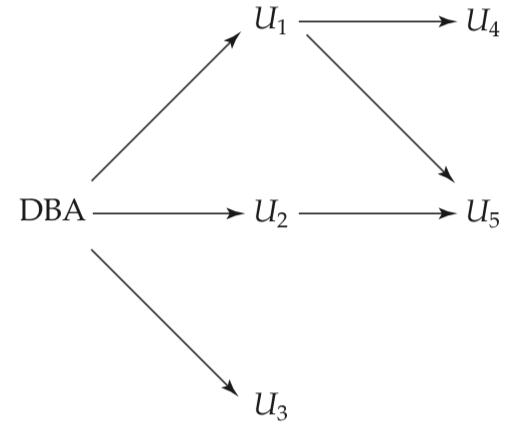
\includegraphics[width=0.35\textwidth]{images/auth-graph}\\
A sample authorization graph~\cite{dsc}.
\end{center}

The graph can be checked for the existence of privileges; a user $U$ has a privilege $p$ if and only if there exists some path from the root (DBA account or root user) to $U$ (however many steps that takes). This is probably inefficient though, as searching the tree on every transaction to see if the user doing the command has permission to do it is likely to take too long. 

What the graph is actually for is revocation. If in the diagram, $U_{1}$ has the permission revoked by the DBA, the permission that $U_{1}$ has granted to $U_{4}$ and $U_{5}$ will be revoked as well. This, in a practical sense, has no impact on $U_{5}$ because the permission has also been granted to $U_{5}$ by $U_{2}$, but $U_{4}$ can no longer perform the operation.

You might think that you can trick the database: if $U_{8}$ grants the permission to $U_{9}$ and then $U_{9}$ grants it to $U_{8}$, if the database administrator revokes the permission grant to $U_{8}$, what happens? If we just used reference-counting, we would see that these users both have the permissions. But in constructing the graph we would see the problem immediately. In this case there is no path from the root to either $U_{8}$ or $U_{9}$, so authorization is revoked from both people~\cite{dsc}. Keep in mind that there does not actually have to be a permanently maintained graph, but it might be necessary to construct it now and again to check the state.

There is the possibility to modify the revoke command to prevent cascading revocation; in that case just put \texttt{RESTRICT} at the end of the statement. If that is the case, then if the permission has been granted to anyone else (i.e., it would cascade), the revocation will not happen and the system will return an error. The opposite of that is the \texttt{CASCADE} keyword, but it's unnecessary to use it because it is the default behaviour if neither restrict nor cascade is specified~\cite{dsc}.

To add one more wrinkle to this, sometimes we want to grant permission not from the current use but from a particular role. If that is the case, then add \texttt{GRANTED BY CURRENT\_ROLE} to the grant statement. 

Allowing users to grant roles is, in my opinion, fairly dangerous. Users are likely not super well equipped to see the consequences of granting permissions and it is likely better if permissions are centrally granted. That is, a database administrator is responsible for the whole process; if a user wishes to grant some permissions to someone else, that user goes to the DBA and asks that the permissions be granted. This sort of centralized management makes sure that there is an oversight process for who can do what and avoids unexpected behaviour when someone's privileges are revoked (e.g., an employee quits and it means members of that person's team can no longer access the complete data of the application).

\subsection*{SQL Injection}

It turns out that you already know quite a lot about the basics of a SQL injection attack. Recall this XKCD from the previous topic:

\begin{center}
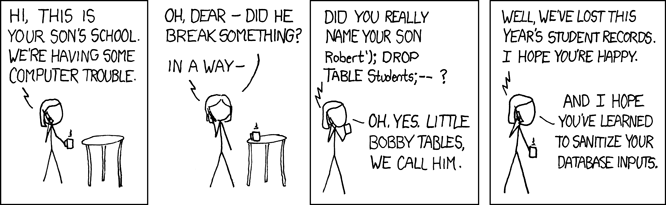
\includegraphics[width=0.7\textwidth]{images/exploits_of_a_mom}\\
Obligatory XKCD ( \url{https://xkcd.com/327/} ).
\end{center}

In short we get into this problem wherever data is entered into the database, usually through an application program. If there is a field for ``name'' we can expect that most users will try to put in their name, but some people will try to break the application. They will try to do this, as above, by putting ending the current statement and then executing an arbitrary statement after that. In the example above,  after the first name there is \texttt{');} to end the previous statement, then the arbitrary command is to drop the table of students, and finally there is a \texttt{-}\texttt{-} which comments out the rest of the line. And with that, the attacker is in, and your data is toast.

There are a few categories of things that can be accomplished by SQL injection~\cite{fds}:

\begin{itemize}
	\item \textbf{SQL Manipulation}: When you put in some SQL statement that adds or changes the conditions of the where-clause or otherwise does some set operation (union, intersect, etc). A common example is adding an \texttt{OR 'x' = 'x'} clause in a where which means the right side condition always returns true.
	\item \textbf{Code Injection}: See the example with little Bobby Tables above: introduce arbitrary SQL statement.
	\item \textbf{Function Call Injection}: Instead of performing a SQL manipulation with the injected command, call a system call or perform some other operating system function (or just make some invalid statements that crash the program... the DB server!).
\end{itemize}

And what can you do with this sort of access~\cite{fds}?
\begin{itemize}
	\item Execute arbitrary commands on the database (as we have seen).
	\item Determine what type of database is in the backend so we can see what is vulnerable.
	\item Denial of service attacks.
	\item Skip authentication (as above).
	\item Learn more about the internal structure of the application (mostly because error pages are very verbose).
	\item Privilege escalation -- gaining access to things that you should not be able to access.
\end{itemize}

In general the solutions are pretty well understood: user input should be filtered (sanitized) and not allowed to be put directly into the queries. This alone might not be enough, and it is better to bind the user input to parameters rather than dynamically building query strings. In this course we don't talk about how to write an application program that interacts with the database (we just tell the database what we want). But do keep this in mind for the future.

\subsection*{Encryption}
As another small note, data encryption is another way to protect your data. Certain sensitive data, such as passwords, must always be kept encrypted in the database. It should be encrypted with a one way hash function. We'll assume that you have some idea about how this works, but basically, if you don't: a security breach means that the passwords of your users will be leaked to the internet. And because users re-use passwords between sites, if someone's password on your service is leaked, it could very easily be someone's online banking password...

With that in mind, encryption keys should also not be stored in the database either... That would make it too easy for attackers! Or, if they are stored in the database, they can be stored encrypted. The standard sort of solution to this is to encrypt the key with the user's password. So the user logs in, the password decrypts the encryption key, and then the encryption key is used to decrypt the sensitive data. This might seem like overkill, but again, you don't want to see your company named and shamed on cable TV as having leaked the personal data of your users, do you?

\bibliographystyle{alphaurl}
\bibliography{356}


\end{document}
